
\mode<presentation>
{
  \usetheme{CambridgeUS}
  \usecolortheme{whale}
  \usecolortheme{lily}

  \setbeamercovered{transparent}
  \usefonttheme[onlymath]{serif}
}

\title[\BodePlotsIIShortName] % (optional, use only with long paper titles)
{\course: \BodePlotsIIName\license}

\subtitle
{Lecture \BodePlotsIINumber} % (optional)


% Delete this, if you do not want the table of contents to pop up at
% the beginning of each subsection:
%\AtBeginSection[]
%{
%  \begin{frame}<beamer>{Outline}
%    \tableofcontents[currentsection,currentsubsection]
%  \end{frame}
%}


% If you wish to uncover everything in a step-wise fashion, uncomment
% the following command:

%\beamerdefaultoverlayspecification{<+->}


\begin{document}

\begin{frame}
  \titlepage
\end{frame}

\mode<article>{
\maketitle
\tableofcontents
}
%\mode<presentation>{
%\begin{frame}{Outline}
%  \tableofcontents
%  % You might wish to add the option [pausesections]
%\end{frame}}

\section{Frequency Response for a Second Order System}

In this lecture, we will see how to sketch an approximate Bode plot for a second order system. First, we plot the exact bode plot to see what it looks like. Our general second order system is parameterized as
\[
G(s) = K\frac{\omega_{n}^{2}}{s^2+2\zeta\omega_{n} s+\omega_{n}^2}
\]
The frequency response function is
\begin{align*}
G(j\omega) &= K\frac{\omega_{n}^{2}}{(j\omega)^2+2\zeta\omega_{n}(j\omega)+\omega_{n}^2}\\
&  = K\frac{\omega_{n}^{2}}{\left(\omega_{n}^{2} - \omega^{2}\right) + j 2\zeta\omega_{n}\omega}
\end{align*}
By dividing top and bottom by $\omega_{n}^{2}$, this can be written as
\begin{equation}
G(j\omega) = K\frac{1}{1 -\left(\frac{\omega}{\omega_{n}}\right)^{2} + j 2\zeta\left(\frac{\omega}{\omega_{n}}\right)}
\label{eq:Gnorm}
\end{equation}
Our first observation:
\begin{itemize}
\item The frequency variable $\omega$ is always divided by the parameter $\omega_{n}$. Just as in the time domain, $\omega_{n}$ acts as a {\em scale factor}. While $\zeta$ may change the shape of the frequency response, $\omega_{n}$ will only stretch or shrink the frequency axis.
\end{itemize}

The magnitude response is the magnitude of $G(j \omega)$ in (\ref{eq:Gnorm}), i.e., 
\begin{align*}
\left|G(j\omega)\right| &= |K|\frac{|1|}{\left|1 -\left(\frac{\omega}{\omega_{n}}\right)^{2} + j 2\zeta\left(\frac{\omega}{\omega_{n}}\right)\right|} \\
&= K \frac{1}{\sqrt{\left(1 -\left(\frac{\omega}{\omega_{n}}\right)^{2}\right)^{2} + \left(2\zeta\frac{\omega}{\omega_{n}}\right)^{2}}}
\end{align*}

The phase response is the phase of of $G(j \omega)$ in (\ref{eq:Gnorm}), i.e., 
\begin{align*}
\angle G(j\omega) & = \angle K + \angle 1 - \angle \left(1 -\left(\frac{\omega}{\omega_{n}}\right)^{2} + j 2\zeta\left(\frac{\omega}{\omega_{n}}\right)\right)\\
& = -  \angle \left(1 -\left(\frac{\omega}{\omega_{n}}\right)^{2} + j 2\zeta\left(\frac{\omega}{\omega_{n}}\right)\right) 
\end{align*}

We can use these magnitude and phase equations to get a qualitative sense of the magnitude and phase Bode plots according to Table~\ref{tab:summary}. 
\begin{table}[h!]
\begin{center}
\caption{Table summarizing magnitude and phase values for three cases of $\omega$ with respect to $\omega_n$ for second order systems. See Appendix A for details. }
\begin{tabular}{clcc}
\toprule
{${\omega}$} & {$|G(j\omega)|$} & {$\angle G(j\omega)$} \\\midrule
\rule{0pt}{12pt} small ( $\ll \omega_n$) & $K$ - constant & $0^{\circ}$ \\
\rule{0pt}{16pt} $=\omega_{n}$ & $\frac{K}{2\zeta}$ & -90$^{\circ}$ \\
\rule{0pt}{16pt}large ( $\gg \omega_n$) & $\frac{K\omega_{n}^{2}}{\omega^{2}}$ - decreasing as $\omega^{2}$ & -180$^{\circ}$\\
\end{tabular}
\label{tab:summary}
\end{center}
\end{table}

By evaluating $|G(j\omega)|$ and $\angle G(j\omega)$ for various values of $\omega$, we can plot the Bode plot. Note that the following plots are scaled so that $K=1$ and $\omega_{n}=1$. We start with the magnitude response, including the actual plot (generated in \textsc{Matlab} using the \texttt{bode} command, plotted in blue) and the linear approximation (red straight lines).

%\begin{frame}{Magnitude Response for Second Order System}
%\begin{center}
%\includegraphics[width=4in]{figures/bodeplot2ndorder}
%\end{center}
%\end{frame}

	\begin{figure}[h!]
	\begin{frame}{Magnitude Response for Second Order System with Linear Approximation}
	\begin{center}
		\begin{tikzpicture}
		\draw (0,0) node {\includegraphics[width=4in]{figures/bodeplot2ndorder}};
		\draw[color=red,line width=3pt] (-3.68,1.2) -- ++(3.9,0);
		\draw[color=red,line width=3pt] (.22,1.2) -- (3.3,-1.4);
		\draw(-2,3) node {$\omega< \omega_{n}$};
		\draw(3,3) node{$\omega > \omega_{n}$};
		\draw(2.5,.5) node{$-40$ \textsf{dB/dec}};
		\draw[thick] (1.35,.3) -- ++(.2,0) -- ++(0,-.16);
		\end{tikzpicture}
	\end{center}
\end{frame}
\caption{Magnitude response with linear approximation for second order system. Note that the break frequency is $\omega_n$ and the high frequency slope is -40 dB/dec.}
\label{fig:magresponse}
\end{figure}


We see in Figure~\ref{fig:magresponse} that the magnitude response has the characteristics that we expected from Table~\ref{tab:summary}: flat at low frequency, inversely proportional to $\zeta$ at $\omega_{n}$, and a decreasing magnitude at high frequency. Although the approximation is not as good as for first order systems, we can still approximate systems with damping ratios greater than 0.4 fairly accurately using the linear approximation.
The approximation is flat until $\omega_{n}$, after which it then decreases by -40 dB/dec. This is double the slope of the first order case: (-20 dB/dec/pole)$\times$(2 poles) = -40 dB/dec. 
Note that the maximum error occurs when $\omega=\omega_{n}$, and can be calculated from $20\log(1/(2\zeta))$. 

Now let's look at the phase response in Figure \ref{fig:phaseresponse}. As with the magnitude plot, the match between the actual frequency response (blue curves) and the linear approximation (red straight lines) varies with $\zeta$, but a good linear approximation is possible when $\zeta>0.4$. 


%\begin{frame}{Phase Response for Second Order System}
%\begin{center}
%\includegraphics[width=4in]{figures/bodeplot2ndorderphase}
%\end{center}
%\end{frame}
%


	\begin{figure}[h!]
\begin{frame}{Phase Response for Second Order System with Linear Approximation}
\begin{center}
\begin{tikzpicture}
\draw (0,0) node {\includegraphics[width=4in]{figures/bodeplot2ndorderphase}};
\draw(-2.5,3) node {$\omega< \frac{\omega_{n}}{10}$};
\draw(.5,3) node{$\frac{\omega_{n}}{10} < \omega < 10\omega_{n}$};
\draw(3.5,3) node{$\omega > 10\omega_{n}$};
\draw[color=red,line width=3pt] (-3.7,1.85) -- ++(1.98,0);
\draw[color=red,line width=3pt] (-1.72,1.85) -- (2.18,-1.1);
\draw[color=red,line width=3pt] (2.18,-1.1) -- ++(1.98,0);
\draw(.55,0.25) node[above right] {$-90^{\circ}$\textsf{/dec}};
\draw[thick] (.4,.3) -- ++(.2,0) -- ++(0,-.16);
\end{tikzpicture}
\end{center}
\end{frame}
\caption{Phase response for second order system. Note that the slope changes significantly as a function of $\zeta$.}
\label{fig:phaseresponse}
\end{figure}

The phase approximation is similar to the first order case (Lecture~\BodePlotsINumber), except that the slope of the decreasing part is -90$^{\circ}$/dec which is double the slope of the first order approximation. Again, you can think of this as each pole having a -45$^{\circ}$/dec slope, so the two poles combined have twice the slope. 

\begin{example} Sketch an approximate Bode plot for the system
\[
G(s) = \frac{2}{s^{2}+10s+25}
\]
\begin{itemize}
\item[Step 1] \textbf{Determine $\omega_{n}$ and $\zeta$}. Comparing the denominator polynomial coefficients to $s^{2}+2\zeta\omega_{n}s + \omega_{n}^2$, we have $\omega_{n} = \sqrt{25} = 5$ and $\zeta = \frac{10}{2\omega_{n}} = 1$
\item[Step 2] \textbf{Determine $K$}. Factoring out the coefficients of the 1s terms, 
\[
G(s) = \frac{2}{25}\frac{1}{\left(\frac{s}{5}\right)^{2} + 2\frac{s}{5} +1}
\]
Thus $K=2/25$
\item[Step 3] \textbf{Plot magnitude plot}.  The low frequency gain will be $20\log_{10}(K)$, and slope of -40 dB/dec after $\omega_{n}$. In this case, the low frequency gain is $20\log_{10}(2/25) = -22$ dB and $\omega_{n}=5$.

\begin{frame}{Magnitude Response}
\begin{center}
\begin{tikzpicture}
\draw (0,0) node {\includegraphics[width=4in]{figures/blankbodeplot}};
\draw[color=red,line width=3pt] (-3.55,2.3) -- ++(3.5,0);
\draw[color=red,line width=3pt] (-.05,2.3) -- (4.6,-1.2);
\draw(2.72,.3) node[above right]{$-40$ \textsf{dB/dec}};
\draw[thick] (2.72,.3) -- ++(.2,0) -- ++(0,-.16);
\end{tikzpicture}
\end{center}
\end{frame}
The max error at $\omega=5$ rad/s is $20\log_{10}(1/2\zeta) = 20\log_{10}(1/2) = -6$ dB. That is, the actual plot will be 6 dB below the linear approximation at $5$ rad/s.
\item[Step 4] \textbf{Plot phase plot}. Since $\omega_{n}=5$, we draw a horizontal line at $0^{\circ}$ until one decade {\em below} 5 rad/s, or 0.5 rad/s, along with a horizontal line at $180^{\circ}$ starting one decade {\em above} 5 rad/s or 50 rad/s. A third line connects these two.
\begin{frame}{Phase Response}
\begin{center}
\begin{tikzpicture}
\draw (0,0) node {\includegraphics[width=4in]{figures/blankbodeplotphase}};
\draw[color=red,line width=3pt] (-3.55,2.45) -- ++(1.45,0);
\draw[color=red,line width=3pt] (-2.1,2.45) -- (2.0,-1.43);
\draw[color=red,line width=3pt] (2.0,-1.43) -- ++(2.7,0);
\draw(-.1,.6) node[above right] {$-90^{\circ}$\textsf{/dec}};
\draw[thick] (-.1,.6) -- ++(.2,0) -- ++(0,-.16);
\end{tikzpicture}
\end{center}
\end{frame}

\end{itemize}
\end{example}

\section{Frequency Response for Other Terms}

\subsection{Frequency Response for Integrators}

Since dividing by $s$ in the Laplace domain is equivalent to integration, a transfer function of the form
\[
G(s) = \frac{K}{s^{n}} 
\]
is called an $n$th order integrator. The frequency response is very simple. Assuming $K>0$, the magnitude response is
\begin{align*}
|G(j\omega)| &= \frac{|K|}{|(j\omega)^{n}|} \\
& = \frac{|K|}{|j\omega|^{n}|}\\
& = \frac{K}{\omega^{n}}
\end{align*}
or, using the properties of logs $\log_{10}(a/b) = \log_{10}a - \log_{10}b$ and  $\log_{10} a^{b} = b\log_{10}a$, 
\[
20 \log_{10}|G(j\omega)| = 20 \log_{10} K - 20 n \log_{10} \omega
\]
in decibels. Since we are plotting on a log scale for $\omega$, this is the equation of a straight line with slope $-20n$ dB/dec, or $-20$ dB/dec for every pole. 


The phase response is
\begin{align*}
\angle G(j\omega) &= \angle \frac{ K }{ (j\omega)^{n}} \\
& = \angle K - n\angle j\omega\\
& = - n 90^{\circ}.
\end{align*}
The phase is thus independent of $\omega$, and the plot will be a horizontal line. 

Plotting the magnitude response can be done in two steps
\begin{itemize}
\item[Step 1] Pick a value of $\omega$, evaluate $20 \log_{10} K - 20 n \log_{10} \omega$ at that frequency, and plot this point on the Bode plot. A particularly convenient value is $\omega = 1$, which as $\log_{10} 1=0$, and the result will be $20\log_{10}K$. 
\item[Step 2] Draw a line of slope $-20n$ dB/dec through this point
\end{itemize}

\begin{frame}{Multiple Integrator Magnitude Response}
\begin{center}
\begin{tikzpicture}
\draw (0,0) node {\includegraphics[width=4in]{figures/blankbodeplotint}};
\draw (1.24,1.05) node[circle,draw,fill,color=red,inner sep=3pt] {};
\draw[color=red,line width=3pt] (-.6,2.2) -- (4.81,-1.2);
\draw(2.55,.3) node[above right]{$-20n$ \textsf{dB/dec}};
\draw[thick] (2.55,.3) -- ++(.2,0) -- ++(0,-.16);
\draw (-5.5,.5) node[rotate=90] {\textsf{Magnitude (dB)}};

\end{tikzpicture}
\end{center}
\end{frame}

The phase response is simply a horizontal line at an angle of -90$n$ degrees.

\begin{frame}{Multiple Integrator Phase Response}
\begin{center}
\begin{tikzpicture}
\draw (0,0) node {\includegraphics[width=4in]{figures/blankbodeplotintphase}};
\draw[color=red,line width=3pt] (-3.9,0.6) -- ++(8.7,0);
\draw (-5.5,.5) node[rotate=90] {\textsf{Phase (degrees)}};
\end{tikzpicture}
\end{center}
\end{frame}

\subsection{Frequency Response for Zeros}

So far, we have looked at systems with one and two poles, but no zeros. Due to the properties of complex numbers, it is easy to find the response for systems with just zeros. Specifically, we know that given complex number $s_{1}=r\angle \theta$ with magnitude $r$ and phase $\theta$, then if 
\[
s_{2} = \frac{1}{s_{1}},
\]
then
\[
s_{2} = \frac{1}{r}\angle (-\theta).
\]
That is, the magnitude is one over the magnitude of $s_{1}$ and the phase is the negative of the phase of $s_{1}$. In addition, if we represent the magnitude in decibels,
\[
20\log_{10}|s_{2}| = 20\log_{10}|1/r| = - 20 \log_{10}|r| = -20\log_{10}|s_{1}|.
\]
Thus, in decibels, the magnitude of $s_{2}$ is {\em also} the negative of the magnitude of $s_{1}$. The following plots illustrate that Bode plots of zeros {\em are the negative of Bode plots of poles}.

\begin{frame}{Comparison of single pole and single zero systems}
\begin{center}
	$G(s) = \frac{\sigma}{s+\sigma} \hspace{1.6in} G(s) = \frac{s+\sigma}{\sigma}$\vspace{.1in}\\<all>
	\includegraphics[width=2.3in]{figures/zerobodeplot1_1}\includegraphics[width=2.3in]{figures/zerobodeplot2_1}\\<all>
	\includegraphics[width=2.3in]{figures/zerobodeplot1_2}\includegraphics[width=2.3in]{figures/zerobodeplot2_2}
\end{center}
\end{frame}

The plots for two pole and two zero systems are also similarly reversed.

\subsection{Frequency Response for Right Half Plane Poles and Zeros}

So far, all of our example systems have had poles and zeros in the left half plane (or, in the case of the integrator, on the imaginary axis). We can look for a symmetry rule to also plot Bode plots for poles and zeros in the right half plane. Poles in the right half plane are called {\em unstable poles}, while zeros in the right half plane are called {\em non-minimum phase zeros}.

What do you observe from the following Bode plots for first order systems with LHP vs. RHP poles?

\newpage
\begin{frame}{Comparison of LHP and RHP pole systems}
\begin{center}
	LHP Pole \hspace{1.7in} RHP Pole \\<all>
	$G(s) = \frac{\sigma}{s+\sigma} \hspace{1.6in} G(s) = \frac{-\sigma}{s-\sigma}$\vspace{.1in}\\<all>
	\includegraphics[width=2.3in]{figures/rhpbodeplot1_1}\includegraphics[width=2.3in]{figures/rhpbodeplot2_1}\\<all>
	\includegraphics[width=2.3in]{figures/rhpbodeplot1_2}\includegraphics[width=2.3in]{figures/rhpbodeplot2_2}
\end{center}
\end{frame}

\begin{frame}
\begin{enumerate}
	\item Are the magnitude plots the same or different? Does this answer make sense given that all we have changed in the transfer function is the sign?
	\item Are the phase plots the same or different? Does this answer make sense given that all we have changed in the transfer function is the sign?
\end{enumerate}
\end{frame}

If you noticed that switching between the LHP and RHP changes the phase plots but not the magnitude plots, and that yes, it makes sense since poles (and zeros) in these two half planes have opposite signs, you're right! In Appendix B, we include some plots and further explanation to explain the details, but here we content ourselves with a summary table:

%\section{Summary}

All of the previous observations are summarized in the following table. 
\begin{frame}
\begin{center}
	\mode<article>{\begin{tabular}{ccccc}
\toprule
Item (Pole/Zero?) & Location & How Many? & Slope of Magnitude & Slope of Phase\\\midrule
\rule{0pt}{12pt}\multirow{5}{*}{Zero} & LHP & 1 & 20 dB/dec & 45$^{\circ}$/dec \\
\rule{0pt}{16pt} & RHP & 1 & 20 dB/dec & -45$^{\circ}$/dec \\%\midrule
\rule{0pt}{16pt} & LHP & 2 & 40 dB/dec & 90$^{\circ}$/dec \\
\rule{0pt}{16pt} & RHP & 2 & 40 dB/dec & -90$^{\circ}$/dec \\
\rule{0pt}{16pt} & $s=0$ (derivative) & $n$ & $20n$ dB/dec & 0$^{\circ}$/dec at 90$n^{\circ}$ \\\midrule

\rule{0pt}{16pt}\multirow{5}{*}{Pole} & LHP & 1 &  -20 dB/dec & -45$^{\circ}$/dec  \\
\rule{0pt}{16pt} & RHP & 1 &  -20 dB/dec &45$^{\circ}$/dec  \\%\midrule
\rule{0pt}{16pt} & LHP & 2 &  -40 dB/dec & -90$^{\circ}$/dec  \\
\rule{0pt}{16pt} & RHP & 2 &  -40 dB/dec &90$^{\circ}$/dec  \\
\rule{0pt}{16pt} & $s=0$ (integrator) & $n$ & $-20n$ dB/dec & 0$^{\circ}$/dec at -90$n^{\circ}$ \\\bottomrule

\end{tabular}
}
	\mode<presentation>{\resizebox{11cm}{!}{\begin{tabular}{ccccc}
\toprule
Item (Pole/Zero?) & Location & How Many? & Slope of Magnitude & Slope of Phase\\\midrule
\rule{0pt}{12pt}\multirow{5}{*}{Zero} & LHP & 1 & 20 dB/dec & 45$^{\circ}$/dec \\
\rule{0pt}{16pt} & RHP & 1 & 20 dB/dec & -45$^{\circ}$/dec \\%\midrule
\rule{0pt}{16pt} & LHP & 2 & 40 dB/dec & 90$^{\circ}$/dec \\
\rule{0pt}{16pt} & RHP & 2 & 40 dB/dec & -90$^{\circ}$/dec \\
\rule{0pt}{16pt} & $s=0$ (derivative) & $n$ & $20n$ dB/dec & 0$^{\circ}$/dec at 90$n^{\circ}$ \\\midrule

\rule{0pt}{16pt}\multirow{5}{*}{Pole} & LHP & 1 &  -20 dB/dec & -45$^{\circ}$/dec  \\
\rule{0pt}{16pt} & RHP & 1 &  -20 dB/dec &45$^{\circ}$/dec  \\%\midrule
\rule{0pt}{16pt} & LHP & 2 &  -40 dB/dec & -90$^{\circ}$/dec  \\
\rule{0pt}{16pt} & RHP & 2 &  -40 dB/dec &90$^{\circ}$/dec  \\
\rule{0pt}{16pt} & $s=0$ (integrator) & $n$ & $-20n$ dB/dec & 0$^{\circ}$/dec at -90$n^{\circ}$ \\\bottomrule

\end{tabular}
}}
\end{center}
\end{frame}

Now that we've seen how different poles and zeros can impact the Bode plot, we'll be able to use information in the Bode plot to better understand systems we want to model. We'll also be able to use the knowledge we've gained in these two lectures to design controllers and filters (even if we're mostly generating the Bode plots in \textsc{Matlab} instead of sketching them by hand). 
%\textcolor{red}{add some stuff about Bode plot interpretation}


\section{Lecture Highlights}
The primary takeaways from this article include
\begin{enumerate}
\setlength{\itemsep}{5pt}
\setlength{\parskip}{0pt}
\setlength{\parsep}{0pt}
\item The sinusoidal steady state magnitude and phase can be evaluated across a range of frequencies and plotted on two log-scale plots; the result is called a \textit{Bode plot}.
\item The Bode plot can be used to quickly evaluate the sinusoidal steady state response of a dynamic system to a sinusoidal input frequency.
\item There are asymptotic rules for sketching Bode plots by hand that depend on the number and locations of poles and zeros; this article gives an example of the rules for $2^{nd}$ order systems with left-half plane (LHP) poles and pure integrators (poles at $s=0$) only.
\item We first derived the asymptotic rules for sketching Bode plots by hand for $2^{nd}$ order systems with left-half plane (LHP) poles and for pure integrators. Then, for LHP zeros, the slopes for both magnitude and phase are flipped compared to those of LHP poles. Furthermore, for RHP poles and zeros, the slopes of the phase plot - but not the magnitude plot - are flipped compared to their LHP counterparts.
%\item \textcolor{red}{We can add magnitude and phase Bode plots of $1^{st}$ and $2^{nd}$ order systems on log scale plots to find the Bode plots for higher order systems. An alternative method for this is given in the next lecture. }

\end{enumerate}

\section{Appendix A: Details for Summary Table}
In this appendix, we show the math that led to qualitative summary in Table~\ref{tab:summary}. In particular, we are looking at the three cases: $\omega \ll \omega_{n}$, $\omega=\omega_{n}$, and  $\omega \gg \omega_{n}$. 
\begin{itemize}
	\item $\omega \ll \omega_{n}$, or $\frac{\omega}{\omega_{n}} \ll 1$. Then
	\[
	|G(j\omega)| \approx K \frac{1}{\sqrt{(1-0)^2 + (2\zeta 0)^2}} = K,
	\]
	and
	\[
	\angle G(j\omega) = -\angle \left( 1 - 0 + j 2\zeta (0)\right) = -\angle 1 = 0.
	\]
	%
	\item $\omega = \omega_{n}$ or $\frac{\omega}{\omega_{n}}=1$. Then
	\begin{align*}
	|G(j\omega)| & = |G(j\omega_{n})|= K \frac{1}{\sqrt{\left(1 -\left(\frac{\omega_{n}}{\omega_{n}}\right)^{2}\right)^{2} + \left(2\zeta\frac{\omega_{n}}{\omega_{n}}\right)^{2}}} \\
	& = K \frac{1}{\sqrt{0 + \left(2\zeta\right)^{2}}}\\
	& = K \frac{1}{2\zeta}\\
	\end{align*}
	and
	\begin{align*}
	\angle G(j\omega) &= \angle G(j\omega_{n}) =-  \angle \left(1 -\left(\frac{\omega_{n}}{\omega_{n}}\right)^{2} + j 2\zeta\left(\frac{\omega_{n}}{\omega_{n}}\right)\right)  \\
	& = -\angle \left( 0 + j 2 \zeta \right)\\
	& = -90^{\circ}
	\end{align*}
	%
	\item $\omega \gg \omega_{n}$, or $\frac{\omega}{\omega_{n}} \gg 1$. Then
	\begin{align*}
	|G(j\omega)| &\approx K\frac{1}{\sqrt{\left(0 - \left(\frac{\omega}{\omega_{n}}\right)^{2}\right)^{2} + \left(2\zeta\frac{\omega}{\omega_{n}}\right)^{2}}}\\
	&= K\frac{1}{\sqrt{\left(\frac{\omega}{\omega_{n}}\right)^{4} + \left(2\zeta\frac{\omega}{\omega_{n}}\right)^{2}}}\\
	& \approx K\frac{1}{\left(\frac{\omega}{\omega_{n}}\right)^{2}}
	\end{align*}
	and
	\begin{align*}
	\angle G(j\omega) & = - \angle \left( -\left(\frac{\omega}{\omega_{n}}\right)^{2} + j 2\zeta\left(\frac{\omega}{\omega_{n}}\right)\right)\\
	& \approx - \angle \left( -\left(\frac{\omega}{\omega_{n}}\right)^{2}\right)\\
	& = -180^{\circ}
	\end{align*}
\end{itemize}

\section{Appendix B: More Information on Right Half Plane Poles and Zeros}

\begin{frame}{Right half plane poles and zeros}
\begin{center}
	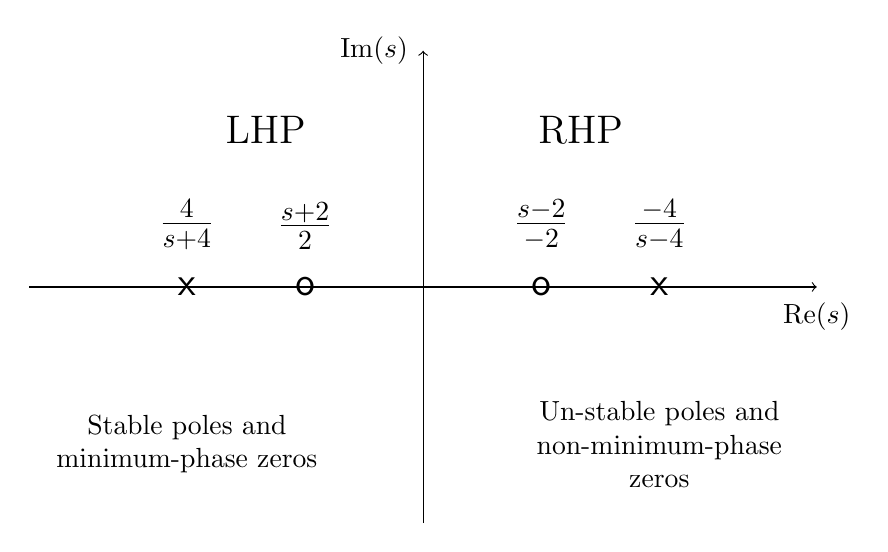
\begin{tikzpicture}

\draw[->] (-5,0) -- (5,0) node[below=2pt] {Re$(s)$};
\draw[->] (0,-3) -- (0,3) node[left=2pt] {Im$(s)$};
\draw (-2,2) node {\Large LHP};
\draw (2,2) node {\Large RHP};
\draw (-3,-2) node {\begin{minipage}{1.5in}\centering Stable poles and minimum-phase zeros\end{minipage}};
\draw (3,-2) node {\begin{minipage}{1.5in}\centering Un-stable poles and non-minimum-phase zeros\end{minipage}};
\draw (-3,0) node (p1) {\Large\sf x};
\draw (p1) node[above=10pt] {\Large$\frac{4}{s+4}$};
\draw (-1.5,0) node (z1) {\Large\sf o};
\draw (z1) node[above=10pt] {\Large$\frac{s+2}{2}$};
\draw (1.5,0) node (z2) {\Large\sf o};
\draw (z2) node[above=10pt] {\Large$\frac{s-2}{-2}$};
\draw (3,0) node (p2) {\Large\sf x};
\draw (p2) node[above=10pt] {\Large$\frac{-4}{s-4}$};
\end{tikzpicture}
\end{center}
\end{frame}

The frequency response for the stable pole is given by
\[
G(j\omega) = \frac{1}{\frac{j\omega}{\sigma} +1},
\]
while the frequency response for the unstable pole is given by
\[
G(j\omega) = \frac{1}{\frac{j\omega}{-\sigma} +1}.
\]
Let's compare $\frac{j\omega}{\sigma}+1$ and $\frac{j\omega}{-\sigma}+1$ in the complex plane

\begin{frame}{Comparison of terms in LHP and RHP}
\begin{center}
\begin{minipage}{2.7in}\begin{tikzpicture}

\draw[->] (-1,0) -- (5,0) node[below=2pt] {Re$(s)$};
\draw[->] (0,-3) -- (0,3) node[left=2pt] {Im$(s)$};
\draw[-o] (0,0) -- (3,2) node[above right] {$\frac{j\omega}{\sigma}+1$};
\draw[-o] (0,0) -- (3,-2) node[below right] {$\frac{-j\omega}{\sigma}+1$};
\draw (3,-.1) node[below] {$1$} -- (3,.1);
\draw (-.1,2) node[left] {$\frac{j\omega}{\sigma}$} -- (.1,2);
\draw (-.1,-2) node[left] {$\frac{-j\omega}{\sigma}$} -- (.1,-2); 
\end{tikzpicture}\end{minipage}\begin{minipage}{2in}\large\centering Same magnitude, but opposite phase\end{minipage}
\end{center}
\end{frame}

Conclusion: for a RHP pole, the magnitude plot is the {\em same} but the phase plot is {\em negative}. The same conclusion holds for a RHP zero.


\section{Quiz Yourself}

\subsection{Questions}

\begin{enumerate}
\setlength{\itemsep}{5pt}
\setlength{\parskip}{0pt}
\setlength{\parsep}{0pt}
\item Draw the approximate Bode plot for the following system
\[
G(s) = \frac{100}{s^2+5s+100}
\]
\item  Sketch the Bode plot for the  system
\[
G(s)= \frac{7}{s^2+4s+4}.
\]
what is the error between your sketch and the actual bode plot at the break frequency?
\item Draw the approximate Bode plot for the following system
\[
G(s) = \frac{s^2+3s+16}{1}
\]
\item  Sketch the Bode plot for the  system
\[
G(s)= \frac{-1}{s-20}.
\]
\end{enumerate}
\newpage
\subsection{Solutions}
\begin{enumerate}
\setlength{\itemsep}{5pt}
\setlength{\parskip}{0pt}
\setlength{\parsep}{0pt}
\item \rule{12pt}{0pt}
\begin{center}
\includegraphics[width=5in]{quizfigures/1asoln}\\
\includegraphics[width=5in]{quizfigures/1bsoln}
\end{center}
\newpage
\item \rule{12pt}{0pt}
\begin{center}
\includegraphics[width=5in]{quizfigures/2asoln}\\
\includegraphics[width=5in]{quizfigures/2bsoln}
\end{center}
\item \rule{12pt}{0pt}
\begin{center}
	\includegraphics[width=5in]{quizfigures/1asoln}\\
	\includegraphics[width=5in]{quizfigures/1bsoln}
\end{center}
\newpage
\item \rule{12pt}{0pt}
\begin{center}
	\includegraphics[width=5in]{quizfigures/2asoln}\\
	\includegraphics[width=5in]{quizfigures/2bsoln}
\end{center}
\end{enumerate}


\end{document}


